\documentclass[x11names]{article}
\usepackage{tikz}
\usepackage{pgfplots}
\usepackage{xcolor}
\usepackage{svg}
\usepackage{amsmath}
\usepackage{array}
\usepackage[skins]{tcolorbox}
\usepackage[version=4]{mhchem}
\usepackage[a4paper, total={6in, 10in}]{geometry}
%\usepackage{fouriernc}
\usepackage{xymtex}
\usepackage{textcomp}
\usepackage{eurosym}
\usepackage{mathrsfs}
\usepackage{float}
\usepackage{pst-all}
\usepackage{pst-3dplot}
\usepackage{leftindex}
\usepackage{verbatim}
\usepackage{import}
\usepackage{xifthen}
\usepackage{pdfpages}
\usepackage{transparent}
\usepackage{import}
\usepackage{pdfpages}
\usepackage{transparent}
\usepackage{amssymb}



\definecolor{myblue}{RGB}{224, 245, 255} 
\definecolor{myred}{RGB}{234, 222, 255}

% box
\newtcolorbox{es}[2][]{%
	enhanced,colback=white,colframe=black,coltitle=black,
	sharp corners,boxrule=0.4pt,
	fonttitle=\itshape,
	attach boxed title to top left={yshift=-0.5\baselineskip-0.4pt,xshift=2mm},
	boxed title style={tile,size=minimal,left=0.5mm,right=0.5mm,
		colback=white,before upper=\strut},
	title=#2,#1
}

% definizioni
\newtcolorbox{blues}[2][]{%
	enhanced,colback=myblue,colframe=black,coltitle=black,
	sharp corners,boxrule=0.4pt,
	attach boxed title to top left={yshift=-0.5\baselineskip-0.4pt,xshift=2mm},
	boxed title style={tile,size=minimal,left=0.5mm,right=0.5mm,
		colback=myblue,before upper=\strut},
	title=#2,#1
}

% teoremi
\newtcolorbox{redes}[2][]{%
	enhanced,colback=myred,colframe=black,coltitle=black,
	sharp corners,boxrule=0.4pt,
	fonttitle=\itshape,
	attach boxed title to top left={yshift=-0.5\baselineskip-0.4pt,xshift=2mm},
	boxed title style={tile,size=minimal,left=0.5mm,right=0.5mm,
		colback=myred,before upper=\strut},
	title=#2,#1
}


%% regole
\renewcommand*\contentsname{Indice}
\setcounter{tocdepth}{4}
\setcounter{secnumdepth}{2}
\pgfplotsset{compat=1.15}


\usetikzlibrary{arrows}


\title{Letteratura italiana}
\author{Federico Cesari}
\date{}



\begin{document}
	
	\begin{titlepage}
	\begin{center}
		\vspace*{1cm}
		
		\textbf{\LARGE Relazione di laboratorio - Pendolo semplice}
		
		\vspace{0.3cm}
		\large \textit{Misura del periodo di un pendolo semplice} \\
		
		\vspace{0.5cm}
		\Large Federico Cesari \\
		
		\small 1096759 
		\vspace{0.2cm}
		
		\small Gruppo 5
		
		
		\vspace{3cm}
		\begin{center}
			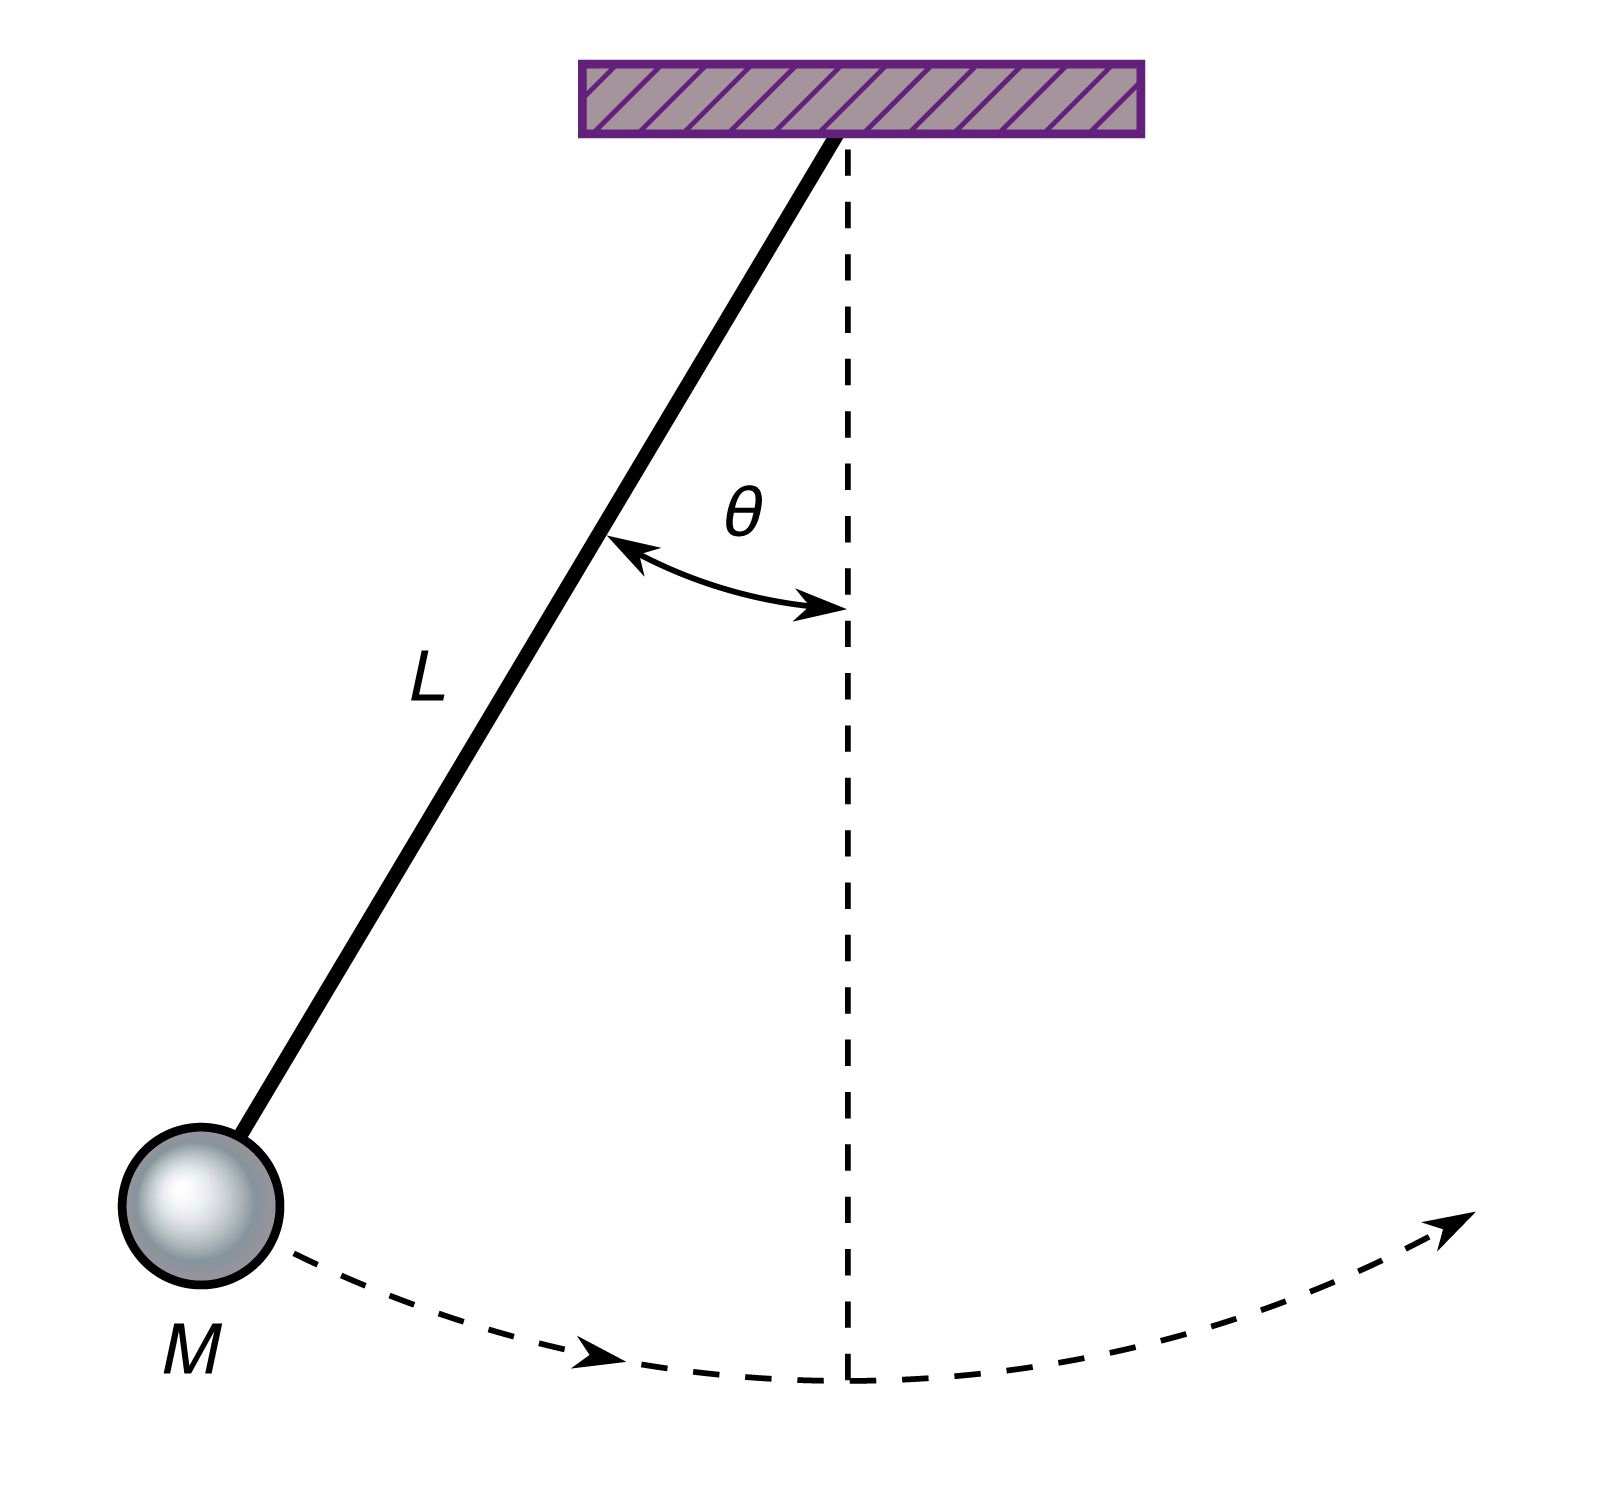
\includegraphics[scale=0.1]{IMG_0200.jpeg}	
		\end{center}
		
		
		
		\vfill
		
		
		
		corso A\\
		Università degli studi di Torino, Torino\\
		4 aprile 2024\\
		
		
	\end{center}
\end{titlepage}
	\tableofcontents
	\newpage
	
	\section{Numeri Complessi}
	L'insieme dei numeri reali può essere esteso con le proprietà delle operazioni di somma e prodotto valide in esso. L'estensione dà vita all'insieme dei numeri complessi che chiamiamo $\mathbb{C}$.
	
	\definecolor{ffqqqq}{rgb}{1,0,0}
	\definecolor{ududff}{rgb}{0.30196078431372547,0.30196078431372547,1}
	\definecolor{wwqqcc}{rgb}{0.4,0,0.8}
	\definecolor{xdxdff}{rgb}{0.49019607843137253,0.49019607843137253,1}
	\begin{center}
		\begin{tikzpicture}[line cap=round,line join=round,>=triangle 45,x=1cm,y=1cm]
			\begin{axis}[
				x=1cm,y=1cm,
				axis lines=middle,
				ymajorgrids=true,
				xmajorgrids=true,
				xmin=-4,
				xmax=4,
				ymin=-4,
				ymax=4,
				ylabel={$i$ }]
				\clip(-9.378848871433435,-6.592409255268999) rectangle (14.57608973860068,7.7305174854563585);
				\draw [->,line width=1pt,color=xdxdff] (0,0) -- (2,1);
				\draw [->,line width=1pt,color=wwqqcc] (0,0) -- (-1,1);
				\draw [->,line width=1pt,color=ffqqqq] (0,0) -- (1,2);
				\begin{scriptsize}
					\draw[color=xdxdff] (1.5040736302530822,0.529963157831875) node {$|z|$};
					\draw [fill=xdxdff] (2,1) circle (2.5pt);
					\draw[color=xdxdff] (2.692438731011955,1.3586914517821413) node {$z (2,i)$};
					\draw [fill=xdxdff] (0,0) circle (2.5pt);
					\draw [fill=wwqqcc] (-1,1) circle (2.5pt);
					\draw[color=wwqqcc] (-1.4512027387393769,1.5306916637340835) node {$w(-1,i)$};
					\draw[color=wwqqcc] (-0.7475655080268867,0.561235923641319) node {$|w|$};
					\draw [fill=ududff] (1,2) circle (2.5pt);
					\draw [fill=ffqqqq] (1,2) circle (2.5pt);
					\draw[color=ffqqqq] (1.066254908920866,2.4845110209221257) node {$z+w$};
					\draw[color=ffqqqq] (1.081891291825588,1.3117823030679754) node {$|z+w|$};
				\end{scriptsize}
			\end{axis}
		\end{tikzpicture}       
	\end{center}
	
	Questo ampliamento permette la risoluzione di qualsiasi equazione algebrica. Il Teorema Fondamentale dell'algebra afferma che qualsiasi polinomio a coefficienti reali o complessi di grado $n, n \in \mathbb{N}$ ammette almeno una radice complessa, da cui segue che un qualsiasi polinomio a coefficienti reali o complessi di grado $n$ ammette sempre $n$ radici complesse contate con le relative molteplicità.
	\\ \\
	\noindent
	I numeri complessi possono essere indicati con tre differenti notazioni: 
	\begin{enumerate}
		\item Cartesiana: $z = (x + iy)$
		\item Trigonometrica: $z = \rho(\cos{\theta} + i\sin{\theta})$
		\item Esponenziale: $z = \rho e^{i\theta}$
	\end{enumerate}
	
	\noindent
	Ogni notazione ha i suoi vantaggi grafici o di calcolo, per questo preferiremo una notazione ad un'altra in casi specifici. In generale un numero complesso è formato dal una \textit{parte reale $x = Re(z)$} e da una \textit{parte immaginaria $y=Im(z)$}, dal punto di vista algebrico $\mathbb{R} $ e $ \mathbb{C}$ hanno le stesse proprietà anche se nel caso dei numeri complessi non è possibile definire un "ordine" compatibile con le operazioni.
	
	\subsection{Operazioni algebriche}
	Le operazioni di somma e differenza sono definite dalla semplice somma o differenza tra parti reali e parti immaginarie. Il prodotto tra due numeri complessi si comporta in modo simile al comportamento di seno e coseno nelle operazioni di somma:
	$$
	z_1 z_2 = (x_1, y_1)(x_2, y_2) = (x_1 x_2 - y_1 y_2, x_1 y_2 + y_1 x_2)
	$$
	
	\vspace{0.7em}
	\noindent
	
	
	
	Il reciproco di un numero complesso espresso come $\frac{1}{z}$ si può riscrivere moltiplicando sopra e sotto per il complesso coniugato di $z = x - iy$:
	
	\[
	\frac{1}{z}\frac{\overline{z}}{\overline{z}} = \frac{x-iy}{x^2 + y^2}
	\]
	
	Nel caso di potenze di un numero complesso la notazione esponenziale è particolarmente funzionale. In generale $z^n$ eleva alla $n$ il modulo $\rho$ e l'argomento:
	
	\[
	z^n = \rho^n e^{in\theta} =  \rho^n(\cos{n\theta} + i\sin{n\theta}) 
	\]
	
	\begin{center}
		\fboxsep11pt
		\colorbox{myblue}{\begin{minipage}{5.75in}
				Un fatto interessante che spiega perché la parte immaginaria dei numeri complessi è situata a $90^\circ$ in senso antiorario rispetto alla parte reale è che se moltiplichiamo un qualsiasi numero complesso per $i$, questo subirà una rotazione di $90^\circ$ in senso antiorario.
				\begin{blues}{es}
					Prendiamo $z= 2+i$ e $w=i$:
					ora $z \cdot w = (2+i)(i)$  sappiamo essere uguale a $-1 + 2i$.
					\begin{center}
						\definecolor{qqwwzz}{rgb}{0,0.4,0.6}
						\definecolor{wwqqcc}{rgb}{0.4,0,0.8}
						\definecolor{xdxdff}{rgb}{0.49019607843137253,0.49019607843137253,1}
						\begin{tikzpicture}[line cap=round,line join=round,>=triangle 45,x=1cm,y=1cm]
							\begin{axis}[
								x=1cm,y=1cm,
								axis lines=middle,
								ymajorgrids=true,
								xmajorgrids=true,
								xmin=-5,
								xmax=5,
								ymin=-5,
								ymax=5,
								ylabel={$i$}]
								\clip(-7.079913199747649,-3.637084505116807) rectangle (8.353685115497054,5.590837202953786);
								\draw[line width=0.8pt,color=qqwwzz,fill=qqwwzz,fill opacity=0.1] (0.6371452110745517,0.31857260553727584) -- (0.31857260553727584,0.9557178166118275) -- (-0.31857260553727584,0.6371452110745517) -- (0,0) -- cycle; 
								\draw [->,line width=1pt,color=xdxdff] (0,0) -- (2,1);
								\draw [->,line width=1pt,color=wwqqcc] (0,0) -- (-1,2);
								\draw [shift={(0,0)},line width=0.8pt,color=qqwwzz] (26.56505117707799:0.7123500017505747) arc (26.56505117707799:116.56505117707799:0.7123500017505747);
								\draw [shift={(0,0)},line width=0.8pt,color=qqwwzz] (26.56505117707799:0.6619792500689667) arc (26.56505117707799:116.56505117707799:0.6619792500689667);
								\begin{scriptsize}
									\draw [fill=xdxdff] (2,1) circle (2.5pt);
									\draw[color=xdxdff] (2.399862266730984,1.3143603851852632) node {$z (2,i)$};
									\draw [fill=wwqqcc] (-1,2) circle (2.5pt);
									\draw[color=wwqqcc] (-0.4813447294569957,2.351997869826389) node {$z_1 (-1,2i)$};
									\draw[color=qqwwzz] (0.9189621672917079,0.6293181623153938) node {$\theta = 90^\circ$};
								\end{scriptsize}
							\end{axis}
						\end{tikzpicture}    
					\end{center}
					
					Sappiamo anche che moltiplicare per $i$ è equivalente a moltiplicare per un certo numero complesso $\cos{\frac{\pi}{2}} + i\sin{\frac{\pi}{2}}$; da ciò notiamo che l'argomento $\theta$ è anche l'angolo di rotazione di un qualsiasi altro numero complesso $l$ moltiplicato per $w$, ovvero per $i$.
					\\\\
					Quindi possiamo decidere di che angolo traslare qualsiasi numero complesso scegliendo opportunamente l'argomento $\theta$ di un altro numero complesso da moltiplicare.
				\end{blues}
		\end{minipage}}        
	\end{center}
	
	%% LOGICA
	\newpage
	\section{Logica}
	\subsection{Proposizioni}
	Definiamo una \textit{proposizione logica} è un enunciato del quale si può inequivocabilmente dire  se  è vero o falso. Attraverso le proposizioni logiche possiamo ottenere operazioni logiche espresse da simboli specifici detti \textit{connettivi logici}: 
	
	\[
	\text{negazione logica}\qquad    \neg p \text{("non p")}\\ \\
	\]
	\[
	\text{congiunzione logica}\qquad   p \wedge q  \text{("p e q")}\\ 
	\]
	\[
	\text{disgiunzione logica}\qquad   p \vee q  \text{("p o q")}\\ 
	\]
	
	\vspace{0.7em}
	\noindent
	In matematica molti enunciati sono del tipo "se $p$ è vera, è vera anche $q$" in cui $p$ è condizione sufficiente affinché $q$ sia vera; in questo caso che $q$ sia vera è condizione necessaria affinchè lo sia anche $p$. Questi tipi di enunciati sono detti implicazioni logiche:
	\[
	\text{implicazione logica}\qquad   p \Rightarrow q  \text{("p implica q")}\\ 
	\]
	\[
	\text{biimplicazione logica}\qquad   p \Longleftrightarrow q  \text{("p equivale a q")}\\ 
	\]
	
	\vspace{0.7em}
	\noindent
	Vengono poi definite delle regole per \textit{negare} le implicazioni o per scriverle in modo logicamente equivalente (nella loro forma \textit{contronominale}):
	
	\[
	\text{contronominale}\qquad   (p \Rightarrow q) \Longleftrightarrow (\neg q \Rightarrow \neg p)  
	\]
	
	\subsection{Predicati}
	Un predicato logico è un enunciato dipendente da uno o più argomenti ed è indicato nella forma $p(x,\dots)$. Gli argomenti $x,\dots$ da cui dipende il predicato rendono quest'ultimo una \textit{proposizione logica} e assume valori di verità Vero o Falso a seconda dei valori assegnati agli argomenti.
	
	\begin{es}{es}
		Dato il predicato "$p(x)$ è un numero dispari" con $x \in \mathbb{N}$:
		
		$p(7)$ è Vero, $p(4)$ è Falso.
	\end{es}
	
	\vspace{0.7em}
	\noindent
	Dato un predicato $p(x)$ con $x \in \mathbb{A}$ è naturale chiedersi se l'enunciato $p(x)$ sia vero \textit{per ogni} elemento di A. A questo fine introduciamo dei \textit{quantificatori}:
	
	\[
	\forall x, p(x) \qquad \text{("per ogni x, è vero p(x)")}  
	\]
	\[
	\exists x, p(x) \qquad \text{("esiste almeno un x, per cui è vero p(x)")}  
	\]
	\[
	\exists !x, p(x) \qquad \text{("esiste, ed è unico, almeno un x, per cui è vero p(x)")}  
	\]
	
	\vspace{0.7em}
	\noindent
	Anche con in quantificatori sono definite le forme di negazione:
	
	\[
	\neg(\forall x, p(x)) \Longleftrightarrow \exists x, \neg p(x)  
	\]
	\[
	\neg(\exists x, p(x)) \Longleftrightarrow \forall x, \neg p(x)
	\]
	
	\subsection{Principio di induzione}
	Sia $P(n)$ una proprietà che dipende da $n \geq n_0 \geq 0 \quad n,n_0 \in \mathbb{N}$. Ora supponiamo che siano verificate:
	
	\begin{itemize}
		\item $P(n_0)$ è Vero;
		\item $\forall n \geq n_0$, se $P(n)$ è vero, allora $P(n+1)$ è vero.
	\end{itemize}
	
	\noindent
	Allora  $P(n)$ è vero per ogni $n \geq n_0$.
	
	\begin{es}{es}
		Sappiamo che $1+2+3+\dots+n = \frac{n(n+1)}{2}$. Dimostriamo che se e vero per $n$ lo è anche per $n+1$ ($P(n) \Rightarrow P(n+1)$):
		
		\begin{align*}
			1+2+3+\dots+n+n+1 & = \frac{(n+1)(n+1+1)}{2} \\ & = \frac{n^2 + n +2n + 2}{2} \\ & = \frac{n^2 + n}{2} + \frac{2n + 2}{2} \\ &=  \frac{n(n+1)}{2} + n+1 
		\end{align*}
		
	\end{es}
	\vspace{0.7em}
	\noindent
	Quindi in generale il Principio di induzione si usa in questo modo: prima si controlla che $P(n_0)$ sia vero, poi si assume che sia vero anche per un generico $n$ e, usando tale informazione, si dimostra che anche $P(n+1)$ è vero.
	
	\newpage
	\section{Numeri reali}
	L'insieme $\mathbb{R}$ è l'ambiente naturale dell'analisi I, nonostante questo non ne conosciamo la definizione rigorosa(!). Possiamo però riflettere sulle sue proprietà:
	\begin{itemize}
		\item Si dice che $\mathbb{R}$ sia un \textbf{campo ordinato}. Ovvero sono definite le due \textit{operazioni di somma e prototto} ed è definita una \textit{relazione d'ordine} $x \leq y$ compatibile con le operazioni (cosa non possibile nell'insieme $\mathbb{C}$).
		\item $\mathbb{R}$ è un insieme \textbf{completo}, al suo interno sono inclusi anche i numeri irrazionali.
	\end{itemize}
	
	\noindent
	\subsection{Completezza di $\mathbb{R}$}
	
	Possiamo dire colloquialmente che $\mathbb{R}$ riempe la retta. Tramite una formulazione più rigorosa notiamo che, dato un certo intervallo, ogni valore successivo è maggiore di un valore nell'intervallo:
	\subsubsection{Maggioranti e minoranti}
	\noindent
	Sia $A \subseteq \mathbb{R}$, si dice che $A$ è:
	\begin{itemize}
		\item \textit{superiormente limitato se  $\exists b \in \mathbb{R} | x \leq b, \forall x \in A$}; $\longrightarrow$ esiste un \textbf{maggiorante} di A.
		\item inferiormente limitato se $\exists a \in \mathbb{R} | a \leq x, \forall x \in A$;$\longrightarrow$ esiste un \textbf{minorante} di A.
		\item limitato se $\exists a,b \in \mathbb{R} | a \leq x \leq b, \forall x \in A$;
	\end{itemize}
	
	\noindent
	Maggiorante e minorante se esistono sicuramente non sono unici: $a,b$ sono infatti ricercati in tutto $\mathbb{R}$; qualunque numero maggiore di un elemento in $A$ è maggiorante e stessa cosa per il minorante.
	
	\subsubsection{Intervalli, massimi e minimi}
	\begin{itemize}
		\item Gli intervalli $(-\infty,b) $ e $ (-\infty,b]$ sono limitati superiormente;
		\item Gli intervalli $(b, +\infty) $ e $ [b, +\infty)$ sono limitati inferiormente;
		\item Gli intervalli $(a,b) $ , $ [ab)$ $(a,b) $ , $ [ab]$ sono limitati.
	\end{itemize}

	
	\begin{center}
		\fboxsep11pt
		\colorbox{myblue}{\begin{minipage}{5.75in}
				\begin{blues}{Definizione: massimio e minimo}
					Sia $A \subseteqq \mathbb{R}$ superiormente (o inferiormente) limitato.
					Si dice che A ammette \textbf{massimo} se
					\[
					\exists x_M \in A \quad \text{ t.c.} \quad x \leq x_M, \quad \forall x \in A
					\]
					\[
					\left(\exists x_M \in A \quad \text{ t.c.} \quad x_M \leq x, \quad \forall x \in A\right)
					\]
					L'elemento, necessariamente unico, si dice \textbf{massimo} (o minimo)  di A e si pone 
					\[
					x_M = \text{ max}A 
					\]
					\[
					\left(x_M = \text{ min}A \right)
					\]
					La differenza con un maggiorante sta proprio nel fatto che il massimo è contenuto nell'intervallo; la stessa cosa si può dire per i minimi. 
				\end{blues}
		\end{minipage}}       
	\end{center}
	\begin{es}{dimostrazione uncità del massimo (o minimo)}
		Se $x_M = x'_M$ sono entrambi massimo allora si ha
		\[
		x \leq x_M \quad \text{e} \quad x \leq x'_M \quad \forall x \in A
		\]
		e quindi
		\[
		x_M \leq x'_M \quad \text{e} \quad x'_M \leq x_M
		\]
		da cui $x_M = x'_M$.
	\end{es}
	
	Esistono casi che però non ammettono massimi o minimi, per esempio l'insieme $\tilde{A} = \{ \frac{1}{n} | n = 1,2,\dots \}$. Quest'ultimo ha come intervallo $[1,+\infty)$, ha quindi un massimo ma non ammette minimi. In questi casi quando $\neg \exists$ minimo o massimo sarebbe utile poter definire un minorante o maggiorante \textit{ottimale} che vengono definiti rispettivamente come \textit{il più grande dei minoranti e il più piccolo dei maggioranti}. Definiamo allora i concetti di \textit{\textbf{estremo superiore}} ed \textit{\textbf{estremo inferiore}}.
	
		\begin{center}
		\fboxsep11pt
		\colorbox{myred}{\begin{minipage}{5.75in}
				\begin{redes}{}
					\subsubsection{Teorema di completezza di $\mathbb{R}$}
					Se $A \subseteqq \mathbb{R}$ è superiormente (inferiormente) limitato, \textbf{il massimo} (minimo) dell'insieme  dei maggioranti (minoranti) \textbf{esiste sempre}.
				\end{redes}
				\end{minipage}}        
		\end{center}
	\begin{center}
		\fboxsep11pt
		\colorbox{myblue}{\begin{minipage}{5.75in}
				\begin{blues}{Definizione: estremo superiore e inferiore}
				Sia $A \subseteqq \mathbb{R}$  superiormente (inferiormente) limitato.
				
				Si dice estremo superiore (inferiore) di A, e si scrive \textbf{supA} (infA), il più piccolo (grande) dei maggioranti (minoranti) di A = \textbf{estremo superiore} (inferiore).
				\end{blues}
		\end{minipage}}       
	\end{center}
	\subsection{Intorni}
	Un'altra  "struttura" fondamentale di $\mathbb{R}$ è quealla che si basa sul concetto di \textbf{intorno}.
	
	\begin{center}
		\fboxsep11pt
		\colorbox{myblue}{\begin{minipage}{5.75in}
				\begin{blues}{Definizione: estremo superiore e inferiore}
					Dati $x_0 \in \mathbb{R}$ e $r > 0$.
					
					Si dice \textbf{intorno} do centro $x_0$ e raggio $r$ l'intervallo 
					\[
					\text{I}_r (x_0) = (x_0 -r, x_0 +r)
					.\]
					Notare che:
					\begin{align*}
						x \in \text{I}_r(x_0) \Longleftrightarrow & x_0 - r < x < x_0 + r \\
						& - r < x -x_0 < r \\
						& |x-x_0| < r
					\end{align*}
					
					
				\end{blues}
		\end{minipage}}       
	\end{center}
	
	\noindent
	Dati $x_0\in \mathbb{R} $ e $ r>0$, si dice intorno di centro $x_0$ e raggio $r$ l'intervallo $In(x_0) = (x_0 -r, x_0 +r)$.
	\\\\
	\noindent
	In questo contesto è utile definire anche un \textit{sistema esteso dei numeri reali} che includa anche $+\infty $ e $ +\infty$: $\overline{\mathbb{R}} = \mathbb{R} \cup \{ -\infty,+\infty \}$. 
	
	\newpage
	\section{Integrali secondo Riemann}
	Il nostro obiettivo è quello di definire un numero reale che rappresenti, quando $f \geq 0$, l'area della regione compresa tra il grafico di $f$ e l'asse $x$.
	
	
	\noindent
	Per fare ciò definiremo:
	\begin{enumerate}
		\item $\int_{a}^{b}f$ per funzioni a scala;
		\item $\int_{a}^{b}f$ per funzioni qualsiasi.
	\end{enumerate}
	
	\subsection{Funzioni a scala}
		\begin{center}
		\fboxsep11pt
		\colorbox{myblue}{\begin{minipage}{5.75in}
				\begin{blues}{Definizione: funzione a scala}
					Una funzione $f: [a,b] \to \mathbb{R}$ si dice a scala se:
					\begin{enumerate}
						\item esistono $n+1$ punti $x_0,x_1, \dots, x_n, x_n$ tali che
						\[
						a = x_0 < x_1 < \dots < x_n =b
						\]
						\item $n$ costanti $c_1, c_2 , \dots , c_n \in \mathbb{R}$
					\end{enumerate}
					 per cui
					 \[
					 f(x) = c_K \quad \forall x \in (x_{k-1}, x_k) \quad k=1,\dots,n
					 \]
				\end{blues}
		\end{minipage}}       
	\end{center}
	
		\begin{center}
		\fboxsep11pt
		\colorbox{myblue}{\begin{minipage}{5.75in}
				\begin{blues}{Definizione: Integrale di funzioni a scala}
					Sia $f \in \mathcal{S}\left(\left[a,b\right]\right)$ (insieme delle funzioni a scala) e sia $x_0, x_1, \dots, x_n$ una suddivisione adattata di $f$ ($f$ continua in ogni sottointervallo).  Detto $c_k$ il valore di $f$ su $\left(x_{k-1}, x_k\right)$ $k=1,\dots,n$:
					
					si dica integrale di $f$ su $\left[a,b\right]$ il numero
					\[
					\sum_{k=1}^{n}c_k (x_k - x_{k-1}) \quad \text{denotato con } \int_{a}^{b}f
					\]
				\end{blues}
		\end{minipage}}       
	\end{center}
	Osserviamo che se $f$ è positiva nell'intervallo il numero $\int_{I}^{}f$ rappresenta l'area del trapezoide di $f$.  \\ \\
	
	\begin{center}
		\fboxsep11pt
		\colorbox{myred}{\begin{minipage}{5.75in}
				\begin{redes}{}
					\subsubsection{Lemma 1: monotonia dell'integrale di funzione a scala}
					Siano $g,h \in \mathcal{S}\left(\left[a,b\right]\right)$ t.c. $g(x) \leq h(x)$ $\forall x \in \left[a,b\right]$, allora:
					\[
					\int_{a}^{b}g \leq \int_{a}^{b}h 
					\]
				\end{redes}
		\end{minipage}}        
	\end{center}
	\begin{es}{dimostrazione}
		Sia $\left\{x_0, x_1, \dots, x_n\right\}$ adattata sia a $g$ sia ad $h$ e siano $c_k$ e $d_k$ i valori di $g$ e $h$ su $\left(x_{k-1},x_k\right)$ con $k=1,\dots,n$. Allora:
		\[
		\int_{a}^{b}g = \sum_{k=1}^n c_k\left(x_k,x_{k-1}\right) \leq \sum_{k=1}^n d_k\left(x_k,x_{k-1}\right) = \int_{a}^{b}h 
		\]
	\end{es}
	\subsection{Integrale superiore e inferiore}
		\begin{center}
		\fboxsep11pt
		\colorbox{myblue}{\begin{minipage}{5.75in}
				\begin{blues}{Definizione: integrale superiore e inferiore}
					Siano 
					\[
					\mathcal{S}^-f = \left\{g \in \mathcal{S}\left(\left[a,b\right]\right) | g(x) \leq f(x) \quad \forall x \in [a,b]\right\}
					\]
					\[
					\mathcal{S}^+f = \left\{h \in \mathcal{S}\left(\left[a,b\right]\right) | f(x) \leq h(x) \quad \forall x \in [a,b]\right\}
					\]
					gli insiemi delle funzioni a scala formati dalle funzioni che \textbf{maggiorano} e \textbf{minorano} $f$.\\ \\
					Nota: $\mathcal{S}f^- \neq \varnothing $ e $\mathcal{S}f^+ \neq \varnothing$ perché \textbf{$f$ è limitata}.
					\[
					\underline{\int_{a}^{b}}f \text{ = integrale inferiore } = \text{sup}\left\{\int_{a}^{b}g \quad \text{t.c.} \quad g \in \mathcal{S}^-f\right\}
					\]
					\[
					\overline{\int_{a}^{b}}f \text{ = integrale superiore } = \text{inf}\left\{\int_{a}^{b}h \quad \text{t.c.} \quad h \in \mathcal{S}^+f\right\}
					\]
				\end{blues}
		\end{minipage}}       
	\end{center}
	
	\begin{center}
		\fboxsep11pt
		\colorbox{myred}{\begin{minipage}{5.75in}
				\begin{redes}{}
					\subsubsection{Lemma 2: integrale inferiore $\leq$ integrale superiore}
					Per ogni funzione $f$ limitata su $\left[a,b\right]$ si ha che l'integrale inferiore è minore o uguale all'integrale superiore:
					\[
					\overline{\int_{a}^{b}}f \leq \underline{\int_{a}^{b}}f
					\]
				\end{redes}
		\end{minipage}}        
	\end{center}
	\begin{es}{dimostrazione}
		Prendo:
		\[
		g \in \mathcal{S}^-f, \quad h \in \mathcal{S}^+f
		\]
		Si ha $g(x) \leq f(x) \leq h(x) \quad \forall x \in [a,b]$. In particolare $g(x) \leq h(x) \quad \forall x \in [a,b]$ e quindi per il \textbf{lemma 1}:
		\[
		\int_{a}^{b}g \leq \int_{a}^{b}h 
		\]
		
		Ora \textit{fisso} $g$ e faccio variare $h$:
		\[
		\int_{a}^{b}g \quad \leq \quad \text{inf}\left\{\int_{a}^{b}h \quad \text{t.c.} \quad h \in \mathcal{S}^+f\right\} \quad = \quad \overline{\int_{a}^{b}}f
		\]
		Ora facendo variare $g$ e ricordando la definizione di integrale inferiore si ottiene la tesi:
		\[
		\underline{\int_{a}^{b}}f \quad \leq \quad \text{sup}\left\{\int_{a}^{b}g \quad \text{t.c.} \quad g \in \mathcal{S}^-f\right\} \quad = \quad \overline{\int_{a}^{b}}f
		\]
		\[
		\Longrightarrow 	\int_{a}^{b}g \leq \int_{a}^{b}h 
		\]
		\end{es}
	\begin{es}{}
		\begin{es}{!attenzione}
			Sembrerebbe logico pensare che la disuguaglianza sopra sia in realtà un'uguaglianza per tutte le funzioni limitate.
			Se prendiamo per esempio la funzione di Dirichlet ci accorgiamo che non è così: $f(x) = \begin{cases}
				1 \quad x \in \mathbb{Q} \\
				0 \quad x \in \mathbb{R} \backslash \mathbb{Q}
			\end{cases}$
			e prendiamo $[a,b] = [0,1]$ abbiamo:
			\[
			\text{se } g \in \mathcal{S}^-f \text{, allora} \quad g(x) \leq 0
			\]
			\[
			\text{se } h \in \mathcal{S}^+f \text{, allora} \quad h(x) \geq 0
			\]
		\end{es}
	\end{es}
	
	A questo proposito diamo la definizione di \textbf{funzione integrabile} secondo \textbf{Riemann}:
		\begin{center}
		\fboxsep11pt
		\colorbox{myblue}{\begin{minipage}{5.75in}
				\begin{blues}{Definizione: Funzione integrabile secondo Riemann}
					Sia $f:[a,b] \to \mathbb{R}$ \textbf{limitata} (condizione necessaria). Si dice che $f$ sia integrabile su $[a,b]$ se
					\[
					\underline{\int_{a}^{b}}f = \overline{\int_{a}^{b}}f 
					\]
					In tal caso si scrive che
					\[
					f \in \mathcal{R}\left(\left[a,b\right]\right)
					\]
					e si pone $\int_{a}^{b}f = \underline{\int_{a}^{b}}f = \overline{\int_{a}^{b}}f$ che si dice \textbf{integrale di $f$ su $[a,b]$}.
				\end{blues}
		\end{minipage}}       
	\end{center}
	
	\newpage
	\section{Limiti e continuità}
	Nel capitolo precedente abbiamo introdotto il concetto di \textit{intorno}, ora vediamo come questo sia essenziale nella comprensione dei \textbf{limiti}.
	
	
	\begin{center}
		\fboxsep11pt
		\colorbox{myblue}{\begin{minipage}{5.75in}
				\begin{blues}{Definizione: Limite}
					Si dice che $\lim_{x\to x_0}f\left(x\right) = l$ se e solo se: 
					\[\forall \text{ intorno di } l, \text{I}\left(l\right) \quad \exists \text{intorno di } x_0, \text{I}\left(x_0\right) \text{ tale che }
					\]
					\[
					\quad x \in I\left(x_0\right) \backslash\{x_0\} \quad \Rightarrow \quad f\left(x\right) \in I\left(l\right)
					\]
				\end{blues}
		\end{minipage}}       
	\end{center}
	
	
	
	
	Adesso dobbiamo stabilire alcune proprietà del limite: intanto se esiste il limite \textit{è unico}, possiamo dire infatti "il limite di $f$" e non "uno dei limiti di $f$".
	
	\begin{center}
		\fboxsep11pt
		\colorbox{myred}{\begin{minipage}{5.75in}
				\begin{redes}{}
					\subsubsection{Teorema di unicità del limite} Supponiamo che $f$ ammetta limite $l$ finito o infinito per $x$ tendente a $x_0$. Allora $f$ non ha altri limiti tendenti a $x_0$.
				\end{redes}
		\end{minipage}}        
	\end{center}
	
	
	\begin{es}{dimostrazione: unicità del limite} 
		Supponiamo che esistano due limiti differenti di una funzione $f$ tendente allo stesso valore $x_0$ e li chiamiamo $l_1$ e $l_2$ tali che $\lim_{x\to x_0}f\left(x\right) = l_1$ e $\lim_{ x\to x_0}f\left(x\right) = l_2$. Inoltre prendiamo gli intorni di  $l_1$ e di $l_2$ in modo che $l_1 \cap l_2 = \varnothing$.
		
		\begin{center}
			\includesvg[scale=1.3]{figures/intornielle}
		\end{center}
		
		
		Ora dalla definizione di limite data prima, possiamo scrivere:
		\begin{enumerate}
			\item $\lim_{x\to x_0}f\left(x\right) = l_1 \quad \Rightarrow \quad  \exists \text{I}\left(x_0\right) | x \in \text{I}\left(x_0\right) \backslash \{x_0\} \quad \Rightarrow \quad f\left(x\right) \in \text{I}\left(l_1\right)$
			\item $\lim_{x\to x_0}f\left(x\right) = l_2 \quad \Rightarrow \quad  \exists \text{I}'\left(x_0\right) | x \in \text{I}'\left(x_0\right) \backslash \{x_0\} \quad \Rightarrow \quad f\left(x\right) \in \text{I}\left(l_2\right)$
		\end{enumerate}
		Dunque possiamo dire che $x$ è sia in $\text{I}(x_0)$ sia in $\text{I}'(x_0)$:
		\[
		x \in \left(\text{I}(x_0) \cap \text{I}'(x_0)\right)\\ \left\{x_0\right\} \Longrightarrow f(x) \in \text{I}(l_1) \cap \text{I}(l_2)
		\]
		Assurdo poiché
		\[
		\text{I}(l_1) \cap \text{I}(l_2) = \varnothing
		\]
	\end{es}
	
	
	\begin{center}
		\fboxsep11pt
		\colorbox{myred}{\begin{minipage}{5.75in}
				\begin{redes}{}
					\subsubsection{Teorema di permanenza del segno}
					Supponiamo che 
					\[
					\lim_{x \to x_0}f(x) = l \qquad \text{con } l>0 \text{ o } l = +\infty.
					\]
					Allora esiste un intorno di $x_0$
					\[
					\text{I}(x_0) \quad \text{t.c. } \quad f(x) > 0 \quad \forall x \in \text{I}(x_0) \backslash \{x_0\}
					\]
				\end{redes}
		\end{minipage}}        
	\end{center}
	
	\begin{es}{dimostrazione}
		$1) \qquad l \in \mathbb{R}, l > 0 \qquad $ 
		
		\begin{center}
			\includesvg[scale=1.3]{figures/permsegno.svg}
		\end{center}
		
		Prendo un intorno di raggio $\varepsilon$ con $\varepsilon = \frac{l}{2}$: $\text{I}_\varepsilon (l)$. Per definizione di limite
		\[
		\exists \text{I}(x_0) \quad \text{t.c.} \quad x \in \text{I}(x_0) \backslash x_0 \Longrightarrow f(x) \in \text{I}_\varepsilon (l)
		\]
		Quindi in particolare 
		\[
		x \in \text{I}(x_0) \backslash \{x_0\} \Longrightarrow f(x) > \frac{l}{2} > 0
		\]
		
		$2) \qquad l = + \infty \qquad$ 
		\begin{center}
			\includesvg[scale=1.3]{figures/permsegno2}
		\end{center}
		\[
		\forall M > 0 \quad \exists \text{I}{x_0} \qquad \text{t.c} \qquad x \in \text{I}{x_0} \backslash \{x_0\} \Longrightarrow f(x) > M > 0
		\]
	\end{es}
	\paragraph{Corollario del teorema di permanenza del segno}
	Se esiste un intorno di $x_0$ I$(x_0)$ in cui $f(x) \geq 0 \quad \forall x \in$ I$(x_0) \backslash \left\{x_0\right\}$ allora (se esiste), il limite
	\[
	\lim_{x \to x_0}f(x) \geq 0
	\]
	\begin{es}{dimostrazione}
		Supponiamo per assurdo che $\lim_{x \to x_0}f(x) = l < 0$, allora per il \textbf{teorema di permanenza del segno}
		\[
		\exists \text{I}'(x_0) \quad \text{t.c.} \quad f(x) <0 \quad \forall x \in \text{I}(x_0) \backslash \left\{x_0\right\}
		\]
		Allora 
		\[
		x \in \left(\text{I}(x_0) \cap \text{I}'(x_0)\right)\backslash\left\{x_0\right\} \Longrightarrow \begin{cases}
			f(x) \leq 0 \\
			f(x) > 0
		\end{cases}
		\]
		che è assurdo.
	\end{es}
	
	\begin{center}
		\fboxsep11pt
		\colorbox{myred}{\begin{minipage}{5.75in}
				\begin{redes}{}
					\subsubsection{Toerema di esistenza del limite per funzioni monotone}
					Data la funzione
					\[
					f: I \rightarrow \mathbb{R}
					\]
					Prendiamo l'intorno $\text{I} = (a,+\infty), a \in \mathbb{R}$.
					
					Se $f$ è \textbf{monotona} su $\text{I}$, allora esiste il limite $\lim_{x \to +\infty}f(x)$ e 
					\[
					\lim_{x \to +\infty} = 
					\begin{cases}
						\text{sup}f(I) \text{ se f è crescente}  \\
						\text{inf}f(I) \text{ se f è decrescente} 
					\end{cases}
					\]
					(la monotonia è \textbf{condizione sufficiente} per l'esistenza del limite)
				\end{redes}
		\end{minipage}}        
	\end{center}
	
	\begin{es}{dimostrazione}
		Supponiamo che $f$ sia crescente con $l = \text{sup}f(I)$.
		
		$l = + \infty\text{)} \qquad$ Dobbiamo dimostrare che
		\[
		\lim_{x \to + \infty}f(x) = l = + \infty
		\]
		cioè
		\[
		\forall M > 0 \quad \exists k > 0  \qquad \text{t.c.} \quad x > k  \quad \Longrightarrow \quad f(x) > M
		\]
		Poiché la funzione è crescente, vale:
		\[
		x > k \quad \Longrightarrow \quad f(x) \geq f(k) > M
		\]
		$l \in \mathbb{R} \text{)} \qquad$ Dobbiamo dimostrare che 
		\[
		\lim_{x \to + \infty}f(x) = l \in \mathbb{R}
		\]
		cioè
		\[
		\forall \varepsilon > 0 \quad \exists k > 0 \quad \text{t.c.} \quad x>k \quad \Longrightarrow \quad l -\varepsilon < f(x) < l + \varepsilon
		\]
		Prendiamo un $\varepsilon$ arbitrario maggiore di zero. Poiché $l-\varepsilon$ non è maggiorante di $f(x)$ esiste sicuramente un $k$ tale che $f(k) > l - \varepsilon$. Poichè la funzione è crescente:
		\[
		x > k \quad \Longrightarrow \quad f(x) \geq f(k) > l - \varepsilon
		\]
		D'altro canto, poiché $l$ è maggiorante di $f(I)$ sappiamo che la funzione sarà sempre minore di $l$: $f(x) \leq l \quad \forall x \in I$ e quindi possiamo affermare che
		\[
		x > k \quad \Longrightarrow \quad l - \varepsilon < f(x) \leq l < l + \varepsilon
		\]
	\end{es}
	
	
	
	
	\begin{center}
		\fboxsep11pt
		\colorbox{myred}{\begin{minipage}{5.75in}
				\begin{redes}{}
					\subsubsection{Teorema del confronto 1}
					Date due funzioni $f$ e $g$ siano i limiti:
					\[
					\lim_{x \to x_0} f(x)  = l \qquad \lim_{x \to x_0} g(x)  = m \qquad \qquad x_0,l,m \in \mathbb{R}
					\]
					Se esiste un intorno in cui $f$ è minore di $g$: 
					\[
					\text{I}(x_0) \text{  t.c. } \quad f(x) \leq g(x) \quad \forall x \in \text{I}(x_0) \backslash \{x_0\}
					\]
					allora sappiamo che il valore a cui tende $f$ è minore di quello a cui tende $g$:
					\[
					l \leq m
					\]
				\end{redes}
		\end{minipage}}        
	\end{center}
	
	\begin{es}{dimostrazione}
		Prendiamo una terza funzione sicuramente positiva:
		\[
		h(x) = g(x) - f(x) \qquad \to h(x) \geq 0 \quad \forall x \in \text{I}(x_0) \backslash \{x_0\}
		\]
		Allora sappiamo per il \textbf{teorema di permanenza del segno} che il limite di $h(x)$ è sicuramente $\geq 0$ e per il \textbf{teorema fondamentale dell'algebra} che:
		\[
		\lim_{x \to x_0} g(x)- \lim_{x \to x_0} f(x) = m - l
		\]
		quindi:
		\[
		0 \leq  \lim_{x \to x_0} h(x) = \lim_{x \to x_0} g(x)- \lim_{x \to x_0} f(x) = m - l
		\]
	\end{es}
	
	\begin{center}
		\fboxsep11pt
		\colorbox{myred}{\begin{minipage}{5.75in}
				\begin{redes}{}
					\subsubsection{Teorema del confronto 2}
					Date due funzioni con stesso limite $l$ :
					\[
					\lim_{x \to x_0} f(x) = l = \lim_{x \to x_0} h(x)
					\]
					Se esiste un intorno $\text{I}(x_0)$ per il quale 
					\[
					f(x) \leq g(x) \leq h(x) \qquad  \forall x \in \text{I}(x_0) \backslash \{x_0\}
					\]
					allora possiamo affermare che 
					\[
					\lim_{x \to x_0} g(x) = l
					\]
				\end{redes}
		\end{minipage}}        
	\end{center}
	\begin{es}{dimostrazione}
		Nel caso in cui $l = \pm \infty$ basta sapere che
		\[
		f(x) \leq g(x) \to +\infty
		\]
		\[
		g(x) \leq h(x) \to -\infty
		\]
		Se invece $l \in \mathbb{R}$ cerchiamo altri intorni di $x_0$ per $f$ e per $h$; per fare ciò prendiamo $\varepsilon > 0$.
		\[
		\lim_{x \to x_0} f(x) = l \quad \Longrightarrow \quad \exists \text{I}'(x_0) \quad \text{ t.c. } \quad \forall \text{I}'(x_0) \backslash \{x_0\} \qquad l - \varepsilon < f(x) < l + \varepsilon
		\]
		\[
		\lim_{x \to x_0} h(x) = l \quad \Longrightarrow \quad \exists \text{I}''(x_0) \quad \text{ t.c. } \quad \forall \text{I}''(x_0) \backslash \{x_0\} \qquad l - \varepsilon < h(x) < l + \varepsilon
		\]
		Ora definiamo un terzo intorno che verifica le condizioni precedenti:
		\[
		x \in (\text{I}(x_0) \cap \text{I}'(x_0) \cap \text{I}''(x_0)) \quad \Longrightarrow \quad l - \varepsilon < f(x)\leq g(x) < h(x) < l + \varepsilon
		\]
	\end{es}
	
	
	
	
	
	
	\newpage
	\section{Proprietà globali delle funzioni continue}
	Nei capitoli precedenti ci siamo occupati, mediante il concetto di limite, delle varie proprietà locali di una funzione, ossia proprietà che valgono in un intorno di un punto della retta reale. Ora è necessario parlare di alcune proprietà globali delle funzioni, valide su tutto l'intervallo.
	
	\begin{center}
		\fboxsep11pt
		\colorbox{myblue}{\begin{minipage}{5.75in}
				\begin{blues}{Definizione: Zero di una funzione}
					Data una funzione reale $f$ chiamiamo \textbf{zero} di $f$ ogni punto $x_0 \in$ dom$f$ in cui la funzione si annulla.
				\end{blues}
		\end{minipage}}        
	\end{center}
	
	\begin{center}
		\fboxsep11pt
		\colorbox{myred}{\begin{minipage}{5.75in}
				\begin{redes}{}
					\subsubsection{Teorema di esistenza degli zeri}
					Sia $f:\left[a,b\right] \rightarrow \mathbb{R}$ una funzione \textit{continua} nell'intervallo chiuso e limitato $\left[a,b\right]$. Se la funzione $f$ assume valori di segno discorde agli estremi dell'intervallo, allora esiste uno zero  di $f$ nell'intervallo aperto $\left(a,b\right)$; in formule:
					\[
					f\left(a\right)f\left(b\right) < 0 \quad \Rightarrow \quad \exists c \in \left(a,b\right) : f\left(c\right) = 0
					.\] 
					Inoltre se $f$ è strettamente monotona in $\left[a,b\right]$, allora lo zero è unico nell'intervallo.
				\end{redes}
		\end{minipage}}        
	\end{center}
	\begin{center}
		\includesvg[scale=0.9]{figures/zeri_func}
	\end{center}
	
	\begin{es}{dimostrazione: teorema esistenza degli zeri}
		Supponiamo $f\left(a\right)$ negativo e $f\left(b\right)$ positivo: $f\left(a\right) < 0 < f\left(b\right)$. 
		\\ \\
		Definiamo poi il punto medio $c_0$ e rinominiamo $a$ e  $b$ : $a = a_0$, $b = b_0$, $c_0=\frac{a_0+b_0}{2}$.
		\\
		\noindent
		Una volta calcolato il punto medio abbiamo tre possibilità:
		\begin{enumerate}
			\item Se $f\left(c_0\right) = 0$ il teorema è dimostrato;
			\item Se $f\left(c_0\right) > 0$ allora dovremo cercare lo zero \textit{a sinistra} del punto medio; in questo caso poniamo quindi $a_0 = a_1$ e $c_0=b_1$;
			\item Se $f\left(c_0\right) < 0$ allora dovremo cercare lo zero \textit{a destra} del punto medio; in questo caso poniamo $c_0= a_1$ e $b_0 = b_1$.
		\end{enumerate}
		
		\begin{center}
			\includesvg[scale=0.7]{figures/due_casi_1}
		\end{center}
		Nei casi $2)$ e $3)$ abbiamo costruito un intervallo  $\left[a_1,b_1\right] \subseteq \left[a_0,b_0\right]$ t.c. 
		
		\[
		f\left(a_1\right)<0<f\left(b_1\right) \quad \text{e} \quad b_1-a_1 = \frac{b_0-a_0}{2}
		.\] 
		\\
		\noindent
		Ora iteriamo il procedimento:
		\[
		c_1 = \frac{a_1+b_1}{2} \quad \text{e consideriamo} \quad f\left(c_1\right) = 0, > 0, < 0
		.\] 
		
		Iterando in questo modo possono verificarsi due casi:
		\begin{enumerate}
			\item In un numero finito di passi troviamo lo zero di $f$;
			\item o troviamo una \textit{successione} di intervalli $\left[a_{n},b_{n}\right]$ t.c.
			\[
			\left[a_0,b_0\right] \supseteq \left[a_1,b_1\right] \supseteq \left[a_2,b_2\right] \supseteq \dots \supseteq\left[a_{n}b_{n}\right]
			.\] 
			\[
			\text{con} \quad f\left(a_{n}\right) < 0 < f\left(b_{n}\right)
			.\] 
			\[
			\text{e con } \quad b_{n} - a_{n} = \frac{b_0-a_0}{2^n}
			.\] 
		\end{enumerate}
		
		Osservando come varia la posizione di $a_{n}$ e di $b_{n}$ notiamo che $a_{n}$ o rimane dov'è o si sposta a destra (aumenta), ivece $b_{n}$ o rimane dov'è o si sposta a sinistra (diminuisce). Possiamo allora dire che le succesioni ${a_{n}}$ e ${b_{n}}$ sono rispettivamente monotona crescente e monotona decrescente, limitate rispettivamente in $\left(a \leq a_{n} \leq b\right)$ e in $\left(a \leq b_{n} \leq b\right)$.
		\\ \\
		Proprio perché le due successioni sono \textit{monotone crescenti}, secondo il teorema di esistenza del limite per successioni monotone:
		\[
		\exists \lim_{n\to \infty}a_{n} = c^- \in \left[a,b\right] \qquad \text{e} \qquad \exists\lim_{n\to \infty}b_{n} =c^+ \in \left[a,b\right]
		.\] 
		
	\end{es}
	\begin{es}{}
		
		
		Da ciò segue che:
		\[
		c^+ - c^- = \lim_{n\to \infty}\left(b_{n} - a_{n}\right) = \lim_{n\to \infty}\frac{b-a}{2^n} = 0
		.\] 
		\[
		c^+ = c^-l =: c \in \left[a,b\right]
		.\] 
		Poiché $f$ è \textit{continua}:
		\[
		\lim_{n\to \infty}f\left(a_{n}\right)  = f\left(c\right) = \lim_{n\to \infty}f\left(b_{n}\right)
		.\] 
		Infine ricordando che $f\left(a_{n}\right) < 0 < f\left(b_{n}\right)$ e ricordando il corollario del teorema di permanenza del segno:
		\[
		f\left(a_{n}\right) < 0 < f\left(b_{n}\right) \quad \Rightarrow \quad f\left(c\right) \leq o \leq f\left(c\right)
		.\] 
		\textbf{Dunque $f\left(c\right) = 0$, $c \in \left(a,b\right)$ } 
	\end{es}
	
	\paragraph{Corollario $7.1$}
	Definiamo un intervallo $I \subseteq \mathbb{R}$ e sia $f:I \rightarrow \mathbb{R}$ una funzione continua. Se esistono (finiti o infiniti) i limiti sinistro e destro di $f$ agli estremi di $I$, e se tali limiti hanno segno discorde, allore esiste uno zero di $f$ in $I$ ; tale zero è unico se $f$ è strettamente monotona in $I$.
	\textit{In soldoni: se a sinistra la curva se ne va in basso verso $-\infty$ e a destra se ne va in alto verso $+\infty$ chiaramente dovrà intersecare l'asse $x$ a un certo punto}.
	
	\paragraph{Corollario $7.2$}
	Siano $f$ e $g$ due funzioni continue in $\left[a,b\right]$.  Se $f\left(a\right)<g\left(a\right)$ e $f\left(b\right)>g\left(b\right)$ allora esiste almeno un punto in $\left(a,b\right)$ tale che:
	\[
	f\left(x_0\right) = g\left(x_0\right)
	.\] 
	Inoltre se $f$ è strettamente crescente e $g$ strettamente decrescente in $\left[a,b\right]$ il punto $x_0$ è unico. \textit{In soldoni: presi due punti $a$ e $b$ sull'asse $x$ e ricavati gli intervalli $\left(f\left(a\right),f\left(b\right)\right)$ e $\left(g\left(a\right),g\left(b\right)\right)$ sull'asse $y$ se l'intervallo di $g$ contiene quello di $f$, allora esiste sicuramente un punto $x_0$ in $f$ contenente $f\left(x_0\right)$}
	\begin{center}
		\includesvg[scale=0.9]{figures/corollario_72}
	\end{center}
	
	
	\begin{center}
		\fboxsep11pt
		\colorbox{myred}{\begin{minipage}{5.75in}
				\begin{redes}{}
					\subsubsection{Teorema dei valori intermedi (0.9)}
					Il teorema si concentra sullo studio dell'immagine di una funzione continua definita su un intervallo  della retta reale.
					\\ \\
					Sia $f:\left[a,b\right] \rightarrow \mathbb{R}$ continua. Allora $f$ assume tutti i valori compresi tra $f\left(a\right)$ e $f\left(b\right)$.
					\\
					Ovvero:
					\[
					\forall y \in \left(f\left(a\right),f\left(b\right)\right) \quad \exists c \in \left[a,b\right] : f\left(c\right) = y
					.\] 
				\end{redes}
		\end{minipage}}        
	\end{center}
	\begin{center}
		\includesvg[scale=0.9]{figures/baby.svg}
	\end{center}
	
	\begin{es}{dimostrazione: teorema valori intermedi}
		Se $f\left(a\right) = f\left(b\right)$ non c'è niente da dimostrare.
		\\ \\
		Se invece supponiamo $f\left(a\right) < f\left(b\right)$ e definiamo la funzione costante $g\left(z\right) = y$ prendendo come $y$ un qualsiasi punto compreso tra $f\left(a\right)$ e $f\left(b\right)$, otteniamo subito le seguenti disuguaglianze:
		\[
		f\left(a\right) < y < f\left(b\right)
		.\] 
		\[
		f\left(a\right) < g\left(a\right) \qquad f\left(b\right) > g\left(b\right)
		.\] 
		Notiamo la somiglianza al corollario $7.2$. Secondo il corollario otteniamo in  $\left[a,b\right]$ l'esistenza di un punto $c$ tale che:
		\[
		f\left(c\right) = g\left(c\right) = y
		.\] 
		Il teorema garantisce che l'immagine di $\left[a,b\right]$ contiene almeno l'intervallo chiuso di estremi $f\left(a\right)$ e $f\left(b\right)$ :
		\[
		\left[f\left(a\right),f\left(b\right)\right] \subseteq f\left(\left[a,b\right]\right) \qquad \text{se} \quad f\left(a\right) \leq f\left(b\right)
		.\] 
		La formula equivalente con $f\left(b\right) \leq f\left(a\right)$ è ovvia.
	\end{es}
	
	\paragraph{Corollario $7.3$}
	Il teorema ha come conseguenza importante il fatto che una funzione continua "trasforma intervalli in intervalli": l'immagina di tale funzione $f\left(I\right)$ attraverso l'intervallo è ancora un intervallo.
	
	\begin{es}{dimostrazione: corollario 7.3}
		Presi $y_1 < y_2$ due punti di $f\left(I\right)$ ; allora esistono in $I$ due punti $x_1$ e $x_2$ tali che:
		\[
		f\left(x_1\right) = y_1 \qquad f\left(x_2\right) = y_2
		.\] 
		Supponiamo che $x_1 < x_2$ e consideriamo $f:\left[x_1,x_2\right] \rightarrow \mathbb{R}$ ; per il teorema dei valori intermedi \textbf{sappiamo che} $f$ assume tutti i valori tra $y_1$ e $y_2$.
	\end{es}
	
	
	\begin{center}
		\fboxsep11pt
		\colorbox{myred}{\begin{minipage}{5.75in}
				\begin{redes}{}
					\subsubsection{Teorema di Weierstrass}
					Se $I$ è chiuso e limitato (cioè $I=\left[a,b\right]$ vale il teorema di Weierstrass.
					\\ \\
					Sia $f:\left[a,b\right] \rightarrow \mathbb{R}$ continua. ALlora $f\left(\left[a,b\right]\right)$ è un intervallo chiuso e limitato, cioè:
					\[
					f\left(\left[a,b\right]\right) = \left[m,M\right]
					.\] 
					in cui $m$ e $M$ sono massimo e minimo. Quindi $f$ assume valore massimo, valore minimo e tutti i valori intermedi.
				\end{redes}
		\end{minipage}}        
	\end{center}
	
	
	
	\newpage
	\section{Derivabilità}
	\begin{center}
		\fboxsep11pt
		\colorbox{myred}{\begin{minipage}{5.75in}
				\begin{redes}{}
					\subsubsection{Teorema di dubbia derivabilità}
					Data una funzione continua nell'intervallo $I$ e derivabile in $I \backslash\{x_0\}$
					\[
					f: I \to \mathbb{R} \qquad I \subset \mathbb{R}
					\]
					\begin{itemize}
						\item Se $\exists \lim_{x \to x_0}f'(x) = l$ allora $\exists f'(x_0) = l$;
						\item Se $\exists \lim_{x \to x_0}f'(x) = \{\pm \infty\}$ allora $f$ non è derivabile in $x_0$;
					\end{itemize}
				\end{redes}
		\end{minipage}}        
	\end{center}
	
	\begin{center}
		\fboxsep11pt
		\colorbox{myred}{\begin{minipage}{5.75in}
				\begin{redes}{}
					\subsubsection{Teorema di Fermat}
					Sia $I \subseteq \mathbb{R}$ intervallo, $f: I \to \mathbb{R}$ derivabile in $x_0$ interno ad $I$,
					\[
					\text{Se } x_0 \text{ punto di estremo per } f \Longrightarrow f'(x_0) = 0 
					\]
					\textbf{Nota:} non vale il veceversa poiché la derivata può annullarsi anche in flessi orizzontali.
				\end{redes}
		\end{minipage}}        
	\end{center}
	
	\begin{es}{dimostrazione}
		Supponiamo di avere $x_0$ punto di massimo locale, allora per definizione
		\[
		\exists \text{I}(x_0) \quad \text{t.c.} \quad f(x) \leq f(x_0) \quad \forall x \in \text{I}(x_0) \cap \text{I}
		\]
		Poiché $x_0$ è interno ad $I$ esiste un intorno J$(x_0)$ t.c. $\text{J}(x_0) \subseteq$ I. Allora I$(x_0) \cap$ J$(x_0)$ è un intorno di $x_0$ e 
		\[
		f(x) \leq f(x_0) \quad \forall x \in \left( \text{I}(x_0) \cap \text{J}(x_0)\right) \subseteq \text{I}
		\]
		Ne segue che:
		\[
		\frac{f(x) - f(x_0)}{x - x_0} \begin{cases}
			\leq 0 \quad x> x_0, \quad x \in \left( \text{I}(x_0) \cap \text{J}(x_0) \right)  \\
			\geq 0 \quad x< x_0, \quad x \in \left( \text{I}(x_0) \cap \text{J}(x_0) \right)
		\end{cases}
		\]
		Per il corollario del teorema di permanenza del segno (o per il teorema del confronto) si ha:
		\[
		f'_+ (x_0) = \lim_{x\to x_0}\frac{f(x) - f(x_0)}{x - x_0} \leq 0
		\]
		\[
		f'_- (x_0) = \lim_{x\to x_0}\frac{f(x) - f(x_0)}{x - x_0} \geq 0
		\]
		Ma \textbf{poiché} $f$ è derivabile in $x_0$:
		\[
		f(x_0) = f'_+(x_0) = f'_-(x_0) = 0
		\]
	\end{es}
	
	
	\begin{center}
		\fboxsep11pt
		\colorbox{myred}{\begin{minipage}{5.75in}
				\begin{redes}{}
					\subsubsection{Teorema di Rolle}
					Sia $f: [a,b] \to \mathbb{R}$ continua su tutto l'intervallo $[a.b]$ e derivabile su $(a,b)$. 
					Se
					\[
					f(a) = f(b) \quad \Longrightarrow \quad \exists c \in (a,b) \quad \text{t.c.} \quad f'(c) = 0
					\]
					Vedremo come in realtà Rolle sia semplicemente un caso particolare del teoreme di Lagrange.
				\end{redes}
		\end{minipage}}        
	\end{center}
	\begin{es}{dimostrazione}
		Per il teorema di Weierstrass sappiamo che l'immagine di una funzione in un intervallo chiuso e limitato è un intervallo chiuso e limitato:
		\[
		f([a,b]) =  [m,M]
		\]
		\textbf{Quindi} esistono $x_m$ e $x_M \in [a.b]$ t.c. 
		\[
		f(x_m) = m \quad \text{e} \quad f(x_M) = M
		\]
		cioè $x_m$ e $x_M$ sono punti di minimo e massimo globale. 
		\begin{itemize}
			\item Se $x_m$ e $x_M$ sono interni a $[a,b]$, allora per il teorema di Fermat $f'=0$ in uno almeno uno dei due punti.
			\item Se $x_m$ e $x_M$ sono esterni, allora la funzione è costante e quindi vale $f'=0 \forall c \in [a,b]$.
		\end{itemize}
	\end{es}
	
	\begin{center}
		\fboxsep11pt
		\colorbox{myred}{\begin{minipage}{5.75in}
				\begin{redes}{}
					\subsubsection{Teorema di Lagrange}
					Sia $f: [a,b] \to \mathbb{R}$ continua su tutto l'intervallo $[a.b]$ e derivabile su $(a,b)$. Allora esiste una $c$ che soddisfa
					\[
					f'(c) = \frac{f'(b) - f(a)}{b - a}
					\]
					Ovvero esiste un punto in cui la retta tangente alla curva è parallela alla retta passante per $a$ e $b$. Infatti:
					\begin{itemize}
						\item $\frac{f'(b) - f(a)}{b - a}$ è il coefficiente angolare della retta passante per $(a,f(a))$ e $(b,f(b))$.
						\item $f'(c)$ è il coefficiente angolare della retta tangente  a $f$ in $c$.
					\end{itemize}
				\end{redes}
		\end{minipage}}        
	\end{center}
	\begin{es}{dimostrazione}
		Definiamo una funzione ausiliaria sicuramente continua su $[a,b]$ e derivabile nell'intervallo $(a,b)$ poiché differenza della funzione $f$ che ha per ipotesi tali proprietà:
		\[
		h(x) = f(x) - \frac{f(b) - f(a)}{b - a}(x-a)
		\]
		Tramite la funzione ausiliaria si verifica facilmente che 
		\[
		h(a) = f(a) \qquad h(b) = f(b)
		\]
		Quindi per il teorema di Rolle sappiamo che esiste una $c \in (a,b)$ che soddisfa $h'(c) = 0$. Ma 
		\[
		h'(c) = f'(c) - \frac{f(b) - f(a)}{b - a} \quad = 0
		\]
		\textbf{Quindi}
		\[
		f'(c) = \frac{f(b) - f(a)}{b - a} \quad 
		\]
	\end{es}
	\paragraph{Proposizione} (caratterizazione dele funzioni a derivata nulla)
	Sia I$\subseteq \mathbb{R}$ intervallo e $f: \text{I} \to \mathbb{R}$ derivabile. Allora
	\[
	f'(x) = 0 \quad \forall x \in \text{I} \quad \Longleftrightarrow \quad f \text{ è costante su I}
	\]
	\begin{es}{dimostrazione}
		$\Longleftarrow \qquad$ Ovvia perché il rapporto incrementale è sempre zero quindi anche il limite.
		
		$\Longrightarrow \qquad$ Proviamo che $\forall x_1,x_2 \in$I$(x_1 < x_2)$ si  ha $f(x_1) = f(x_2)$.
		Usiamo il \textbf{teoreme di Lagrange}:
		
		esiste $c \in (x_1,x_2)$ t.c.
		\[
		f(x_2) - f(x_1) = f'(c)(x_2 - x_1)
		\]
		\[
		f(x_2) - f(x_1) = 0 \quad \Longrightarrow \quad f(x_1) = f(x_2)
		\]
	\end{es}
	
	\begin{center}
		\fboxsep11pt
		\colorbox{myred}{\begin{minipage}{5.75in}
				\begin{redes}{}
					\subsubsection{Teorema di Cauchy}
					Siano $f$ e $g$ continue su $[a,b]$ e derivabili su $(a,b)$. Si supponga che $g'(x) \neq 0 \forall x \in (a,b)$, allora esiste sicuramente una
					\[
					c \in (a,b) \quad \text{t.c.} \quad \frac{f'(c)}{g'(c)} = \frac{f(b) - f(a)}{g(b) - g(a)}
					\]
				\end{redes}
		\end{minipage}}        
	\end{center}
	
	
	\section{Taylor}
	Lo sviluppo di Taylor di una funzione nell'intorno di un punto $x_0$ dell'asse reale, è la rappresentazioe come somma di un polinomio e di un infinitesimo di ordine superiore al grado dol polinomio. Con esso è possibile approssimare una funzione complessa (in un intorno abbastanza piccolo di $x_0$) a un polinomio, di cui è facile stabilire le proprietà qualitative.
	
	Iniziamo supponendo una funzione continua in $x_0$ e costante (di grado 0), sappiamo che per $x\to x_0$:
	\[
	f(x) = f(x_0), \quad \forall x \in \mathbb{R}
	\]
	In altri termini possiamo approssimare la funzione $f$ mediante un polinomio di grado 0 in modo che la differenza tra $f(x)$ e $T_{f_0,x_0}(x)$ sia un infinitesimo di $x_0$.
	
	Supponiamo che la funzione sia anche derivabile:
	\[
	f(x) = f(x_0) + f'(x_0)(x-x_0) + o(x-x_0)
	\]
	
	In generale posso trovare il polinomio $T_{n,x_0}(x)$ di grado $leq n$ tale che:
	\[
	f(x) = T_{n,x_0}(x) + o\left( (x-x_0)^n\right)
	\]
	che è riscrivibile come:
	\[
	\lim_{x\to x_0}\frac{f(x) - T_{n,x_0}(x)}{(x-x_0)^n} = 0
	\]
	\begin{center}
		\fboxsep11pt
		\colorbox{myred}{\begin{minipage}{5.75in}
				\begin{redes}{Teorema: formula di Taylor con resto di Peano}
					Sia $f:$I$\to \mathbb{R}$ derivabile n volte in $x_0$, allora posto
					\[
					T_{n,x_0}(x) = \sum_{k=0}^{n}\frac{1}{k!}f^{(k)}(x_0)(x-x_0)
					\]
					risulta
					\[
					f(x) = T_{n,x_0}(x) + o\left( (x-x_0)^n\right) \qquad \text{per }x \to x_0
					\]
					Il polinomio $T_{n,x_0}(x)$ è \textbf{unico} e si chiamo \textbf{polinomio di Taylor di ordine n} (per $x_0 = 0$ si chiamo polinomio di Mac-Lawri)
				\end{redes} 
		\end{minipage}}        
	\end{center}
	\begin{es}{dimostrazione}
		Per $n=0$ e $n=1$ già lo sappiamo. Dimostriamo che per 
		\[
		n = 2 \quad \to \lim_{x\to x_0}\frac{f(x) - T_{2,x_0}(x)}{(x-x_0)^2} = 0
		\]
		dove
		\[
		T_{2,x_0}(x) = f(x_0) + f'(x_0)(x-x_0) + \frac{1}{2}f''(x_0)(x-x_0)^2
		\]
		Per il \textbf{teorema di De L'Hopital} è vero se:
		\[
		\lim_{x\to x_0}\frac{f'(x) - f'(x_0)+f''(x_0)(x-x_0)}{2(x-x_0)} = 0
		\]
		cioè
		\[
		\frac{1}{2}\lim_{x\to x_0}\left( \frac{f'(x) - f'(x_0)}{x-x_0} - f''(x_0)\right) = 0
		\]
		che è vero per la definizione di derivata seconda.
	\end{es}
	
	\newpage
	\section{Primitivazione}
	
	
	\newpage
	\section{Equazioni differenziali}
	
		\begin{center}
		\fboxsep11pt
		\colorbox{myblue}{\begin{minipage}{5.75in}
				\begin{blues}{Definizione: soluzione di *}
					Si dice sluzione di * la funzione
					\[
					y: \text{I} \to \mathbb{R} \quad \text{t.c.} \quad y^{(n) = f(x,y(x),y'(x),\dots,y^(n-1)(x))} \quad \forall x \in \text{I}
					\]
					(con I intervallo) e $f$ derivabile n volte.
				\end{blues}
		\end{minipage}}       
	\end{center}
	
	\begin{es}{esempio 1}
		\[
		y' = g(x) \qquad \left(y'(x) = g(x)\right)
		\]
		Giò risolta (se g è continua).
		\[
		y(x) = G(x) \qquad \qquad G' = h, c \in \mathbb{R}
		\]
	\end{es}
	
	\begin{es}{esempio 2}
		\[
		y' = ky \qquad k \in \mathbb{R}
		\]
		\[
		y(x) = e^{kx} \Longrightarrow y'(x) = ke^{kx} = ky(x)
		\]
		Per trovare le soluzioni, osservo che:
		\begin{align*}
			\left(e^{-kx}y(x)\right)' =& - ke^{-kx}y(x) + e^{-kx}y'(x) \\
			&= \left(y'(x) - ky(x)\right)e^{-kx}
		\end{align*}
		Quindi
		\begin{align*}
			y'(x) = ky(x) \Longleftrightarrow & \left(e^{-kx}y(x)'\right)' = 0 \\
			\Longleftrightarrow & e^{-kx}y(x) = c \\
			\Longleftrightarrow & y(x) = ce^{kx}
		\end{align*}
	\end{es}
	
	\begin{es}{esempio 3}
		\[
		y' = y^2
		\]
		Verifico che $y(x) = - \frac{1}{x+c} \quad c \in \mathbb{R}$ è soluzione:
		\[
		y'(x) = \frac{1}{(x+c)^2} = y(x)^2
		\]
	
		\textit{Fatto interessante}
		\[
		y(x) = - \frac{1}{x+c}
		\]
		è definita su I = $(-\infty, -c)$ o su I= $(-c, + \infty)$.	Il modello prevede un'esplosione (blow-up) in un tempo finito.
	\end{es}
	\begin{es}{esempio 4}
		\[
		y'' = g(x) \qquad \text{g continua}
		\]
		Si ha
		\begin{align*}
			y'(x) &= c_2 \qquad G'=& g, \quad c_2 \in \mathbb{R} \\
			y(x) =& c_1 + c_2x + \mathcal{G}(x) \mathcal{G}' =& G (\mathcal{G}'' = g), \quad c_1, c_2 \in \mathbb{R}
		\end{align*}
		Per $g(x) = -g$ costanti, $\mathbb{G} = - \frac{g}{2}x^2$ e quindi
		\[
		y(x) = c_1 + c_2x - \frac{g}{2}x^2
		\]
		Cinematica: $F(t,s,v) = -mg$ (forza peso)
		\begin{align*}
			ms'' = mg \Longrightarrow & s'' = -g \\
			\Longrightarrow & s(t) = c_1 + c_2t - \frac{g}{2}t^2
		\end{align*}
		che è la legge oraria di caduta dei gravi.
	\end{es}
	
	
	\noindent
	Per determinare una \textbf{unica} soluzione, si impongono condizioni aggiuntive, in questo casso si parla di \textbf{problema di Cauchy}.
	
	\[
	\text{I ordine)} \quad \begin{cases}
		y' = f(x,y) \\
		y(x_0) = y_0 \quad \text{ condizione iniziale}
		\end{cases} 
	\]
	\[
	\text{II ordine)} \quad \begin{cases}
		y'' = f(x,y,y') \\
		y(x_0) = y_0 \quad \text{ posizione iniziale} \\
		y'(x_0) = z_0 \quad \text{ velocità iniziale}
 	\end{cases} 
	\]
	
	\begin{es}{esempio 1}
	\[
		\begin{cases}
			N' = kN  \quad k>0 \\
			N(0) = N_0  > 0 
		\end{cases} 
	\]
	\[
	\Longrightarrow N(t)  = ce^{kt} \quad c \in \mathbb{R} 
	\]
	\[
	\Longrightarrow N(0) = ce^0 = c
	\]
	$(k>0) \qquad \Longrightarrow N(t) = N_0 e^{kt} \quad \forall t \in \mathbb{R}$
	Rappresenta una crescita esponenziale (irrealistica). \\ \\
	
	\noindent
	Il modello logistico invece
	\[
	\begin{cases}
		N' = kN(1 - \frac{N}{h}) \\
		N(0) = N_0
	\end{cases}
	\]
	ha come asintoto il valore della "capacità portante dell'ambiente".
	\end{es}
	\begin{es}{esempio 2}
	\[
	\begin{cases}
		ms'' = -mg \quad \Longrightarrow s(t) = c_1 + c_2t - \frac{g}{2}t^2 \\
		\begin{array}{c}
		s(0) = s_0 \\
		s'(0) = v_0
		\end{array} 
		\Longrightarrow \begin{cases}
							s(0) = c_1 = s_0 \\
							s'(t) = c_2 -gt \quad \Longrightarrow s'(0) = c_2 = v_0
						\end{cases}
	\end{cases} 
	\]
	\\ \\
	$\Longrightarrow s(t) = s_0 + v_0t + \frac{-g}{2}t^2$
	\end{es}
	
	\subsection{Equazioni differenziali del second'ordine}
	\[
	y'' + ay' + by = g(x) \qquad a.b \in \mathbb{R}, \quad g:\text{I} \to \mathbb{R} \text{ continua}
	\]
	L'equazione con $g(x) = 0$, cioè
	\[
	y'' + ay' + by = 0
	\]
	si dice \textbf{omogenea} associata. \\ \\
	
	\noindent
	Perché il termine "lineare"? L'operatore differenziale
	\begin{align*}
		\mathcal{L}_2 =& C^2 \to C^0 \\
		& y \to y'' + ay' + by
	\end{align*}
	è lineare, cioè $\mathcal{L}_2 (c_1y_1 + c2_y2)$ = $c_1 \mathcal{L}_2(y_1) + c_2 \mathcal{L}_2(y_2) \quad \forall c_1, c_2 \in \mathbb{R}, \quad \forall y_1,y_2 \in C^2$ \\ \\
	
	\noindent
	Come conseguenza: se $y_1,y_2$ sono soluzioni di $	y'' + ay' + by = g(x)$, allora $c_1y_1 + c_2y_2$ è anche soluzione, ovvero:
 l'insieme delle soluzioni di 	$y'' + ay' + by = g(x)$ è spazio vettoriale (= il nucleo di $\mathcal{L}$). \\ \\
 
\noindent
Si considera l'equazione caratteristica
\[
\lambda^2 + a \lambda + b = 0, \qquad \lambda \in \mathbb{C}
\]
e distinguiamo 3 casi: posto $\Delta = a^2 - 4b$

\begin{enumerate}
	\item $\Delta 0$: dette $\lambda_{1,2} = - \frac{a}{2} \pm \frac{\sqrt{\Delta}}{2}$ le due soluzioni di (LO2) sono date da 
	\[
	y(x) = c_1 e^{\lambda_1 x} + c_2 e^{\lambda_2 x} 
	\] \\ \\
	
	\noindent
	Infatti 
	\begin{align*}
		D\left(e^{\lambda_i x}\right) =& \lambda_i e^{\lambda_i x} \\ 
		D^2\left(e^{\lambda_i x}\right) =& \lambda_i^2 e^{\lambda_i x} \\ 
	\end{align*}
	\item $\Delta = 0$: detta $\lambda = - \frac{a}{2}$ la soluzione reale (doppia): le soluzioni di (LO2) sono date da 
	\[
	y(x) = \left(c_1 + c_2x\right)e^{\lambda x} \qquad c1, c_2 \in \mathbb{R}
	\]
	\item $\Delta < 0$: date $\lambda_{1,2} = \sigma \pm i \omega$ le due osluzioni complesse coniugate $\left(\sigma = - \frac{a}{2}, \omega = \frac{\sqrt{-\Delta}}{2}\right)$ le soluzioni di (LO2) sono data da
	\[
	y(x) = \left(c_1\cos{\omega x} + c_2 \sin{\omega x}\right) e^{\sigma x} \qquad c_1,c_2 \in \mathbb{R}
	\]
\end{enumerate} 

Nel caso non-omogeneo, e soluzioni sono date da 
\[
y(x) = c_1y_1(x) + c_2y_2(x) + y_p(x) \qquad \text{in cui} y_p \text{ è soluzione particolare dell'eq. completa}
\]
\end{document}



 